\chapter{The Augmented Lagrangian}
Until now there were only two ways to add constraints to the control problem: 1. use a proximal function or 2. add a soft constraint to the cost function. It is up to the user to determine the weights of the soft constraints. Weights that are too high, will result in a badly conditioned problems. Putting the weights too low will result in more violations of the soft constraints.

In order to avoid confusion in this chapter, adding constraints by adding them to the cost function with a fixed weight, will be called the direct method. A alternative method will be introduced in this chapter and referred to as the augmented Lagrangian method.

\section{Definition of the augmented Lagrangian}
	One way to reduce the ill conditioning of the problem when increasing the weights of the soft constraints, is the usage of the augmented Lagrangian as described in Chapter 17 of \cite{Wright}. Furthermore current research done by Ben Hermans at the KuLeuven suggests a way to update the weights or also called the penalty parameters.
	
	\begin{equation}
		\begin{aligned}
			& \underset{x}{\text{argmin}}
			& & f_0(x) \\
			& \text{subject to}
			& & g(x)=0
		\end{aligned}
		\label{eq:opti problem lagrangian}
	\end{equation}
	
	The problem described in \eqref{eq:opti problem lagrangian} can be solved by minimizing \eqref{eq:lagrangian quadratic model}  for x with a fixed $\mu_k$, and then solving again for x with $\mu_{k+1}>\mu_k $. As mentioned before increasing $\mu$ will worsen the condition of the problem. 
	
	\begin{equation}
		Q(x,\mu) \overset{def}{=} f(x) + \mu \sum_{i \in \epsilon} c_i^2(x)
		\label{eq:lagrangian quadratic model}
	\end{equation}
	
	By adding Lagrangian multipliers \eqref{eq:augmented lagrangian definition} is obtained. However the feasibility condition $c_i(x)=0$ will not be met in the first iterations. Each time the problem is solved, the condition of \eqref{eq:perturbed feasibility conditions} is met. As $\mu_k$ goes to infinity the condition of \eqref{eq:perturbed feasibility conditions} will get more similar to that of the feasibility condition.
	
	\begin{equation}
		\Lagr_A(x,\lambda;\mu) \overset{def}{=} f(x) - \sum_{i \in \epsilon}\lambda_ic_i(x) + \mu \sum_{i \in \epsilon}c_i^2(x)
		\label{eq:augmented lagrangian definition}
	\end{equation}
			
	\begin{equation}
		c_i(x_k) = -\lambda_i/\mu_i
		\label{eq:perturbed feasibility conditions}
	\end{equation}
	

\section{Optimality conditions}
	The value of the Lagrangian multiplier can be determined from \eqref{eq:gradient augmented lagrangian definition}. The Lagrangian multipliers are determined trough the optimality condition. Which can be obtained by taking the derivative of the Lagrangian towards x, and putting it to zero.($\nabla_x \Lagr_A(x_k,\lambda_k;\mu_k) = 0$) The gradient will only be zero, if the optimality conditions displayed in \eqref{eq:optimality codition augmented lagrangian definition} are met.
	\begin{equation}
		\lambda_{k+1}^{i} = \lambda_{k}^{i} - 2\mu_k c_i(x_k)
		\label{eq:optimality codition augmented lagrangian definition}
	\end{equation}

	\begin{equation}
		\nabla_x \Lagr_A(x_k,\lambda_k;\mu_k) = \nabla f(x_k) - \sum_{i \in \epsilon} [\lambda_i^k - 2\mu_k c_i(x_k)] \nabla c_i(x_k)
		\label{eq:gradient augmented lagrangian definition}
	\end{equation}	
	
	%\begin{equation}
	%	c_i(x) \approx \frac{1}{\mu_k}(\lambda_{k+1} - \lambda_k)
	%\end{equation}
	
	
\section{Algorithm}
	Algorithm~\ref{alg:PANOC with augmented lagrangian} proposed by ?? Ben Hermans ??, where $0<\beta<1$. Ben Hermans proposes to set $\mu_{k+1}=\mu_k \cdot 2$ if $c_i(x)$ is over a certain predefined tolerance. The idea is, that if a constraint is too badly violated its weight clearly needs to be increased. So when it's solved in the next iteration, it won't be violated as much.
	
	\begin{algorithm}
		\caption{PANOC nmpc with augmented lagrangian}
		\label{alg:PANOC with augmented lagrangian}
		\begin{algorithmic}[1]
			\Procedure {SOLVE\_MPC}{state}
			\State $\mu_0=0$
			\State $\lambda_0=0$
			\While{residual < mpc\_residual }
			\State (residu,input\_horizon) = nmpc\_solve(residual\_solver,state,input\_horizon,$\mu_k$,$\lambda_k$)
			\State $\lambda_{k+1}^{i} = \lambda_{k}^{i} - 2\mu_k c_i(x_k)$
			\State update penality parameter $\mu_{k+1}>\mu_k$
			\State residual\_solver =  residual\_solver$\cdot \beta$
			\EndWhile
			\EndProcedure
		\end{algorithmic}
	\end{algorithm}

\section{Simulation}
In order to illustrate the advantage of the augmented Lagrangian towards a simple soft constraint on the cost function. A simple simulation is set up with two obstacles, using the trailer model. The trainer has to move from the circle towards the star, while avoiding the two circles. The two obstacles, are always added using the direct method. The path taken by the trailer is illustrated in figure~\ref{fig:LA path}.

In addition to the two obstacles a speed limit can be added to the problem. The speed limit can be expressed added using the direction method. Or it can be added using the augmented Lagrangian. The  constraint is mathematically expressed in \eqref{eq:speed limit constraint} with M the maximum allowed speed..

\begin{equation}
\max\{(v_x^2+v_y^2+v_z^2)-M^2,0\}^2
\label{eq:speed limit constraint}
\end{equation}

Figure~\ref{fig:simulation with augmented Lagrangian} contains the simulation results of the same simulation solved without speed limit, with the speed limit as a soft constraint directly onto the cost function. And a simulation using the augmented Lagrangian to add the speed limit constraint.

The optimal constraint violation value is set to 0.1 which means that the augmented Lagrangian algorithm will increase the weight of the speed limit constraint, until the violation of the constraint is under 0.1 . 

Figure~\ref{fig:LA iterations} contains the amount of iterations till convergence in each step of the simulation. Figure~\ref{fig:LA time} contains the time to convergence in each step of the simulation. Figure~\ref{fig:LA time} contains the speed of the trailer at each step in the simulation, the maximum speed is set to one. This means that the speed of the trailer in figure~\ref{fig:LA speed} should never go over one.

From figure~\ref{fig:LA time} it is obvious that without the speed limit the convergence is faster than with either the direct method or with the augmented Lagrangian method. However the augmented Lagrangian method is significantly faster then using a soft constraint.

If the weight of the soft constraint is lowered the direct method can be faster than the augmented Lagrangian method. However if the weight of the soft constraint is lowered, the soft constraint will will be significantly violated. And some sort of trade-off must be made, by the user before hand.

The augmented Lagrangian method however is much easier to set up, as the weight of its constraints is automatically tuned. It also does not suffer as badly from bad conditioning.

\begin{figure}[H]
	\centering
	\begin{subfigure}[b]{0.45\textwidth}
		\centering
		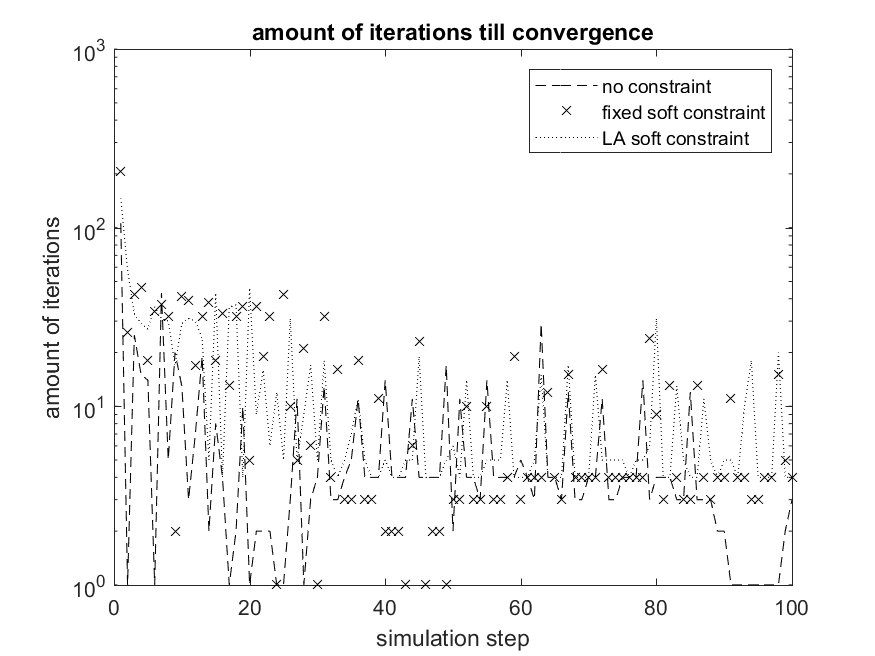
\includegraphics[width=1.2\textwidth]{LA/LA_sim_iterations}
		\caption{iterations}
		\label{fig:LA iterations}
	\end{subfigure}
	\hfill
	\begin{subfigure}[b]{0.45\textwidth}
		\centering
		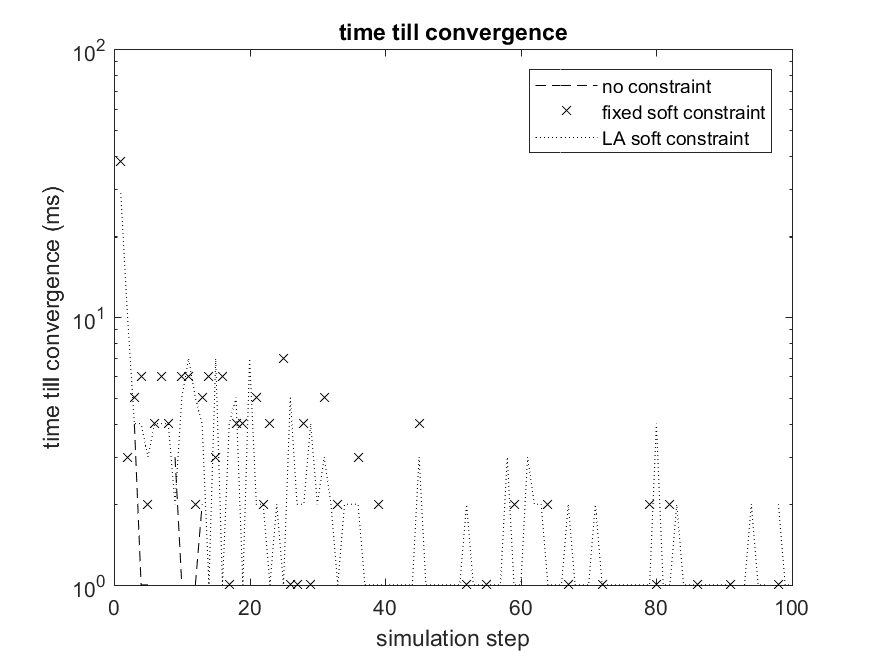
\includegraphics[width=1.2\textwidth]{LA/LA_sim_time}
		\caption{convergence time in each step}
		\label{fig:LA time}
	\end{subfigure}
	\begin{subfigure}[b]{0.45\textwidth}
		\centering
		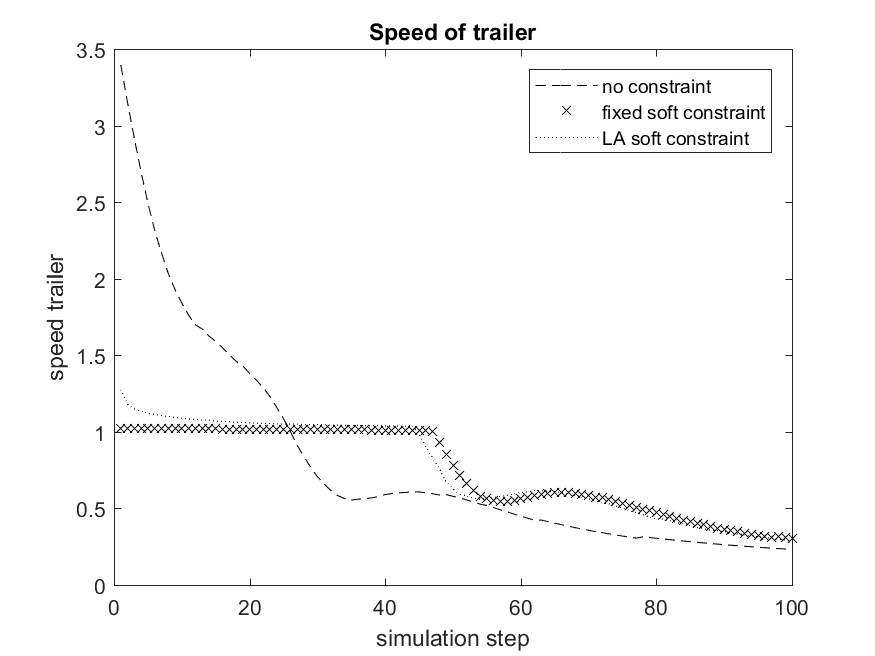
\includegraphics[width=1.2\textwidth]{LA/LA_sim_speed}
		\caption{speed of the trailer in each step}
		\label{fig:LA speed}
	\end{subfigure}
	\hfill
	\begin{subfigure}[b]{0.45\textwidth}
		\centering
		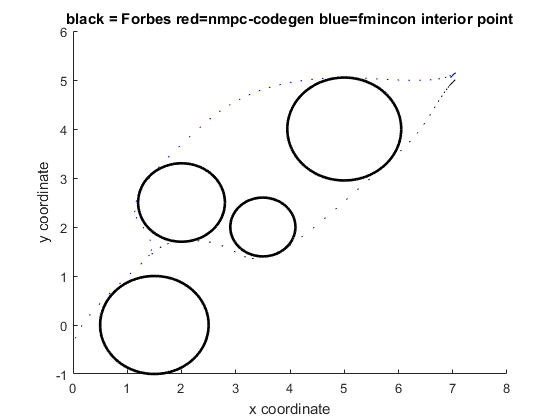
\includegraphics[width=1.2\textwidth]{LA/path}
		\caption{path taken by the trailer without speed limit}
		\label{fig:LA path}
	\end{subfigure}
	\caption{Simulation with augmented Lagrangian}
	\label{fig:simulation with augmented Lagrangian}
\end{figure}
